%%%%%%%%%%%%%%%%%%%%%%%%%%%%%%%%%%%%%%%%%
% NIH Grant Proposal for the Specific Aims and Research Plan Sections
% LaTeX Template
% Version 1.0 (21/10/13)
%
% This template has been downloaded from:
% http://www.LaTeXTemplates.com
%
% Original author:
% Erick Tatro (erickttr@gmail.com) with modifications by:
% Vel (vel@latextemplates.com)
%
% Adapted from:
% J. Hrabe (http://www.magalien.com/public/nih_grants_in_latex.html)
%
% License:
% CC BY-NC-SA 3.0 (http://creativecommons.org/licenses/by-nc-sa/3.0/)
%
%%%%%%%%%%%%%%%%%%%%%%%%%%%%%%%%%%%%%%%%%

%----------------------------------------------------------------------------------------
%	PACKAGES AND OTHER DOCUMENT CONFIGURATIONS
%----------------------------------------------------------------------------------------

\documentclass[11pt,notitlepage]{article}

% Variabili per non ripetere i contatti mille volte, MODIFICARE QUI
\newcommand{\nomeStudente}{Nome}
\newcommand{\cognomeStudente}{Cognome}
\newcommand{\matricolaStudente}{1234567}
\newcommand{\emailStudente}{xxx.yyy@zzz.com}
\newcommand{\telStudente}{+39 0000000000}

\newcommand{\nomeTutorAziendale}{Nome}
\newcommand{\cognomeTutorAziendale}{Cognome}
\newcommand{\emailTutorAziendale}{xxtutor@azienda.it}
\newcommand{\telTutorAziendale}{+39 0000000000}

\newcommand{\ragioneSocAzienda}{Azienda S.p.A.}
\newcommand{\indirizzoAzienda}{Via xxxxxxxxxxx, Padova (PD)}
\newcommand{\sitoAzienda}{http://www.azienda.it}



% A note on fonts: As of 2013, NIH allows Georgia, Arial, Helvetica, and Palatino Linotype. LaTeX doesn't have Georgia or Arial built in; you can try to come up with your own solution if you wish to use those fonts. Here, Palatino & Helvetica are available, leave the font you want to use uncommented while commenting out the other one.
%\usepackage{palatino} % Palatino font
\usepackage[utf8x]{inputenc}%codifica
\usepackage{helvet} % Helvetica font
\usepackage{multirow}
\renewcommand*\familydefault{\sfdefault} % Use the sans serif version of the font
\usepackage[T1]{fontenc}
\linespread{1.2} % A little extra line spread is better for the Palatino font
\usepackage{fancyhdr} %pacchetto per le intestazioni
\usepackage{hyperref}
\usepackage{lipsum} % Used for inserting dummy 'Lorem ipsum' text into the template
\usepackage{amsfonts, amsmath, amsthm, amssymb} % For math fonts, symbols and environments
\usepackage{graphicx} % Required for including images
%\usepackage{booktabs} % Top and bottom rules for table
%\usepackage{wrapfig} % Allows in-line images
%\usepackage[labelfont=bf]{caption} % Make figure numbering in captions bold
\usepackage[top=0.5in,bottom=0.5in,left=0.5in,right=0.5in]{geometry} % Reduce the size of the margin
\pagestyle{empty}

\hyphenation{ionto-pho-re-tic iso-tro-pic fortran} % Specifies custom hyphenation points for words or words that shouldn't be hyphenated at all

\hypersetup{
	colorlinks=true,
	linkcolor=black,
	urlcolor=blue
}

%----------------------------------------------------------------------------------------
%	Creato da Mich - Updated by Simone Pessotto 04/08/2015
%----------------------------------------------------------------------------------------

\begin{document}
	
\noindent
\parbox{0.7\columnwidth}{Università degli Studi di Padova\\
	Piano di lavoro stage presso \ragioneSocAzienda{}\\
	\nomeStudente{} \cognomeStudente{} (\matricolaStudente{})}%matricola
\parbox{0.3\columnwidth}{
	\hfill 
\includegraphics[scale=0.08]{immagini/logo-unipd.png}}

\bigskip
\begin{center}
{\Huge \textbf{Piano di lavoro}} \\ \bigskip
	{\Large \textit{presso \ragioneSocAzienda{}}}\\ \bigskip
	{\Large \textit{\nomeStudente{} \cognomeStudente{}}}
\end{center}

\section*{Contatti}
\textbf{Studente:} \nomeStudente{} \cognomeStudente{}, \href{mailto:\emailStudente{}}{\emailStudente{}}, \telStudente{} \\
\textbf{Tutor aziendale:} \nomeTutorAziendale{} \cognomeTutorAziendale{}, \href{mailto:\emailTutorAziendale{}}{\emailTutorAziendale{}}, \telTutorAziendale{} \\
\textbf{Azienda:} \ragioneSocAzienda{}, \indirizzoAzienda{}, \href{\sitoAzienda{}}{\sitoAzienda{}}

\section*{Scopo dello stage}

L'azienda si occupa di sviluppare prodotti software di GENERE X rivolto a utenti Y.\\

\noindent Lo stage prevede l'inserimento dello studente nel team di programmazione UI/DATABASE/BOH. Lo studente verrà formato nel campo de X, ponendo attenzione alle diverse necessità e soluzioni riscontrabili in un ottica Y.\\ 

\noindent Gli argomenti trattati saranno principalmente:
\begin{itemize}
	\item ARGOMENTO1;	
	\item ARGOMENTO2;	
	\item ARGOMENTO3;	
	\item ARGOMENTO4;
	
\end{itemize}

\newpage

\noindent
\parbox{0.7\columnwidth}{Università degli Studi di Padova\\
	Piano di lavoro stage presso \ragioneSocAzienda{}\\
	\nomeStudente{} \cognomeStudente{} (\matricolaStudente{})}%matricola
\parbox{0.3\columnwidth}{
	\hfill 
\includegraphics[scale=0.08]{immagini/logo-unipd.png}}

\bigskip
\section*{Pianificazione del lavoro}
La pianificazione, in termini di quantità di ore di lavoro, sarà così distribuita:

\begin{center}
	
\begin{tabular}{|l|l|c l|}
	\hline
	\multicolumn{2}{|l|}{\textbf{Durata in ore}}		&	\multicolumn{2}{l|}{\textbf{Descrizione dell'attività}}\\
	\hline
	\multicolumn{2}{|l|}{168}	&	\multicolumn{2}{l|}{Studio e implementazione di X}\\
	\hline
	\multirow{5}{1cm}{ }    &            16            &            \hspace{5mm}•\hspace{2mm}            &       Attività1\\
	\cline{2-2}
	&            40            &           \hspace{5mm}•\hspace{2mm}         &           Attività2\\
	\cline{2-2}
	&            16            &            \hspace{5mm}•\hspace{2mm}            &            Attività3\\
	\cline{2-2}
	&            48            &            \hspace{5mm}•\hspace{2mm}            &            Attività4\\
	\cline{2-2}
	&            48            &         \hspace{5mm}•\hspace{2mm}           &            Attività5\\
	\hline
	
	\multicolumn{2}{|l|}{88}	&	\multicolumn{2}{l|}{Analisi di X}\\
	\hline
	
	\multirow{3}{1cm}{ }    &            16            &            \hspace{5mm}•\hspace{2mm}            &       Attività\\
	\cline{2-2}
	&            32            &            \hspace{5mm}•\hspace{2mm}            &            Attività\\
	\cline{2-2}
	&            40            &         \hspace{5mm}•\hspace{2mm}           &            Attività\\
	\hline
	
	\multicolumn{2}{|l|}{32}	&	\multicolumn{2}{l|}{Studio e utilizzo di X}\\
	\hline	
	
	\multirow{5}{1cm}{ }    &            16            &            \hspace{5mm}•\hspace{2mm}            &            Attività\\
	\cline{2-2}
	&            16            &         \hspace{5mm}•\hspace{2mm}           &            Attività\\
	\hline

	\multicolumn{2}{|l|}{32}	&	\multicolumn{2}{l|}{Studio ed implementazione di X}\\
	\hline
	
	\multirow{5}{1cm}{ }    &            16            &            \hspace{5mm}•\hspace{2mm}            &            Attività\\
	\cline{2-2}
	&            16            &         \hspace{5mm}•\hspace{2mm}           &            Attività\\
	\hline	
\end{tabular}

\end{center}

\section*{Obiettivi}

Si farà riferimento ai requisiti secondo le seguenti notazioni:
\begin{itemize}
	\item «ob» per i requisiti obbligatori, vincolanti in quanto obiettivo primario
	richiesto dal committente;
	\item  «de» per i requisiti desiderabili, non vincolanti o strettamente necessari,
	ma dal riconoscibile valore aggiunto;
	\item «op» per i requisiti opzionali, rappresentanti valore aggiunto non
	strettamente competitivo.
\end{itemize}
Le sigle precedentemente indicate saranno seguite da una coppia sequenziale di numeri, identificativo del requisito.\\

\newpage

\noindent
\parbox{0.7\columnwidth}{Università degli Studi di Padova\\
	Piano di lavoro stage presso \ragioneSocAzienda{}\\
	\nomeStudente{} \cognomeStudente{} (\matricolaStudente{})}%matricola
\parbox{0.3\columnwidth}{
	\hfill 
\includegraphics[scale=0.08]{immagini/logo-unipd.png}}

\bigskip
\bigskip
\noindent
Si prevede lo svolgimento dei seguenti obiettivi:
\begin{itemize}
	\item Obbligatori
	\begin{itemize}
		\item \underline{\textit{ob01}}: studio della struttura di X;
		\item \underline{\textit{ob02}}: studio approfondito delle diverse categorie di Y
		\item \underline{\textit{ob03}}: Z;
		\item \underline{\textit{ob04}}: Z 4 Q Q Q simboloDiBatman;
		\item \underline{\textit{ob05}}: zzzz;
	\end{itemize}
	
	\item Desiderabili 
	\begin{itemize}
		\item \underline{\textit{de01}}: analisi e ricostruzione dello schema di un DB esistente;
		\item \underline{\textit{de02}}: gestione di X;
		\item \underline{\textit{de03}}: gestione di Y;
		\item \underline{\textit{de04}}: comprensione e applicazione di Z;
	\end{itemize}
	
	\item Opzionali
	\begin{itemize}
		\item \underline{\textit{op01}}: comprensione e gestione di Ajeje.
	\end{itemize} 
\end{itemize}


\section*{Diagramma di Gantt}
Di seguito è riportato il diagramma di Gantt relativo al piano di lavoro previsto.
\begin{center}
	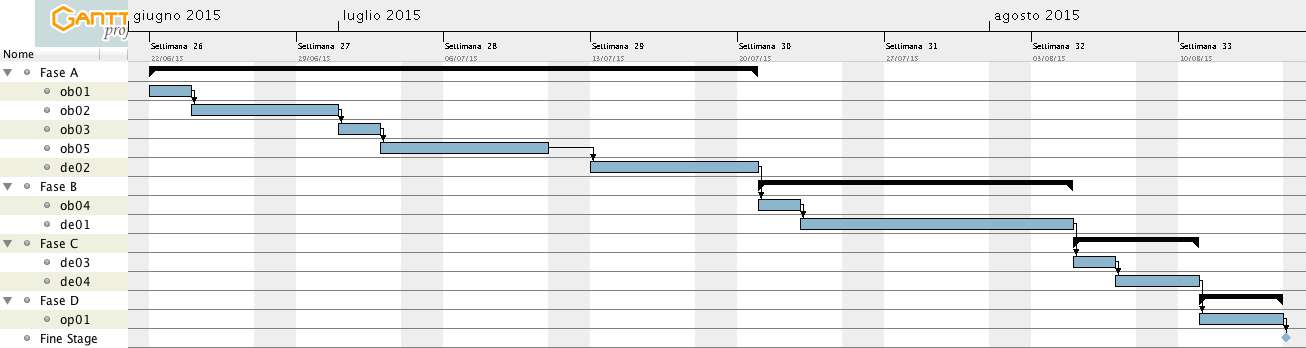
\includegraphics[scale=0.42]{immagini/gantt.png}
\end{center}
\end{document}